\documentclass[12pt]{article}
\usepackage{amsmath}
\usepackage{graphicx}

\usepackage{booktabs} % For \toprule, \midrule and \bottomrule
\usepackage{siunitx} % Formats the units and values
\usepackage{pgfplotstable} % Generates table from .csv
% Setup siunitx:
\sisetup{
	round-mode          = places, % Rounds numbers
	round-precision     = 2, % to 2 places
}

\begin{document}
		\pagenumbering{gobble}
	\title{Maths Mid Term}
	\author{Shruti Ravichandran}
	\maketitle
	\newpage
	\tableofcontents
	\newpage
	{ \begin{center}
			College of Engineering Pune \\Department of Mathematics \\MA-19002 : Univariate Calculus \\End Semester Examination
		\end{center}
	}\raggedleft
	{\bf Date : 8th November 2022      \hspace*{\fill}            Max Marks : 60}
	\\{\bf Branches : All        \hspace*{\fill}                    Semester : 2}	       
	\\\raggedright{\bf Programme : BTech}   

	\pagenumbering{arabic}
	\addcontentsline{toc}{section}{Section A}
	\raggedright\section*{Section A}
	Q1.Solve the equation to obtain roots:
	\begin{equation*}
		x^2+2x+9=0
	\end{equation*}
\\
	Q2.Solve the following inequation and write down the solution set:
	\begin{equation*}
		11x-4<15x+4<=13x+14,x\in W
	\end{equation*}
\\
	Q3.State whether the following differential equations are linear or non linear,justify and solve.
	\begin{equation*}
		a)xy'+2y=e^{3x}/x,x>0 
		b)x^2ydy/dx-xy^2=1 
	\end{equation*}
\\
\addcontentsline{toc}{section}{Section B}
\section*{Section B}
	Q4.Which of the given values of x and y will make the following pairs of matrices equal?
	\begin{equation*}
		\begin{bmatrix}3x+7&5\\y+1&2-3x
		\end{bmatrix}=
		\begin{bmatrix}0&y-2\\8&4
		\end{bmatrix}
	\end{equation*}
	\vspace{0.5cm}
	$\hspace{2cm}a)x=\frac{-1}{3},y=7 \hspace{5cm} b)Not possible\newline \hspace*{1.85cm}$
	$ c)y=7,x=\frac{-2}{3} \hspace{5cm} d)x=\frac{-1}{3},y=\frac{-2}{3}$
	\\
	Q5.Solve the following integral
	\begin{equation*}
		\int_{7}^8 (3x^4+2x+3x^2)dx
	\end{equation*}
	\\
	Q6. Evaluate the limit of the following
	\begin{equation*}
		\lim_{x \to +\infty}\sqrt[3]{x}+12x-2x^2
	\end{equation*}
	Q7.Solve the determinant
	\begin{equation*}
		\begin{vmatrix}3&4&5&9\\1&4&8&9\\2&6&84&6\\7&4&0&2
		\end{vmatrix}	
	\end{equation*}
\addcontentsline{toc}{section}{Section C}
\section*{Section C}

Q8.The distribution in the table below shows the number of wickets taken by bowlers in one-day cricket matches. Find the mean number of wickets using the correct method. What does the mean signify?
\begin{table}[h!]
	\begin{center}
		\caption{}
		\begin{tabular}{l|c} 
			\textbf{Number of wickets} & \textbf{Number of bowlers}\\
			\hline
			20-60 & 7\\
			60-100 &5\\
			100-150 & 16\\
			150-250 & 12\\
			250-300&2\\
			
			
		\end{tabular}
	\end{center}
\end{table}\\
\newpage
Q9.Solve the following puzzle
\vspace{1cm}
\begin{center}
	
	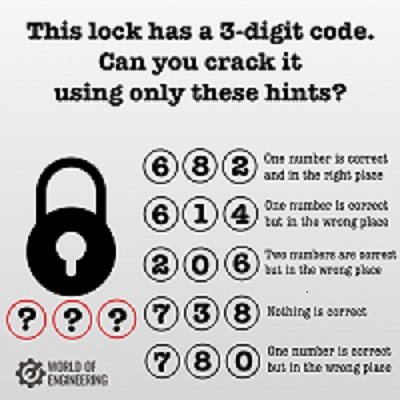
\includegraphics{puzzle.jpg}\\
	
	\label{puzzle}
\end{center}
\vspace{1.5cm}
Q10.Find the median height.
\begin{table}[h!]
	\begin{center}
		\caption{Autogenerated table from .csv file.}
		\label{table1}
		\pgfplotstabletypeset[
		multicolumn names, % allows to have multicolumn names
		col sep=semicolon, % the seperator in our .csv file
		display columns/0/.style={
			column name=$Height$, % name of first column
			column type={S},string type},  % use siunitx for formatting
		display columns/1/.style={
			column name=$Number of girls$,
			column type={S},string type},
		every head row/.style={
			before row={\toprule}, % have a rule at top
			after row={
				\cm & \count\\ % the units seperated by &
				\midrule} % rule under units
		},
		every last row/.style={after row=\bottomrule}, % rule at bottom
		]{table.csv} % filename/path to file
\end{center}
\end{table}
	\newpage
	\section{Differential Equations}
	\subsection{Types}
	\subsubsection{Ordinary Differential Equations.}
	\subsubsection{Partial Differential Equations.}
	\subsubsection{Linear Differential Equations.}
	\subsubsection{Non Linear Differential Equations.}
	\subsubsection{Homogenous Differential Equations.}
	\subsubsection{Non-Homogenous Differential Equations.}
	
\end{document}